\documentclass[12pt, twoside]{report}
\usepackage[a4paper,bindingoffset=0.2in,%
            left=0.8in,right=0.8in,top=1.2in,bottom=1.2in,%
			]{geometry}
\usepackage{graphicx}
\usepackage{subcaption}
\usepackage{caption}
\usepackage{fancyhdr}
\fancyhf{}
\renewcommand{\headrulewidth}{0pt}
\fancyhead[RO,LE]{\thepage}
\pagestyle{fancy}
\setcounter{chapter}{1}
\begin{document}
	\tableofcontents
	
	\newpage
	
% Page no - 5
 
	\chapter{Background and Literature Review}
	\large{The importance of facial expression in social interaction and social intelligence is widely recognized. Facial expression analysis has been an active research topic since 19th century. The first automatic facial expression recognition system was introduced in 1978 by Suwa et al. [83]. This system attempts to analyze facial expressions by tracking the motion of 20 identified spots on an image sequence. Since then, a lot of work has been done in this domain. Various computer systems have been made to help us understand and use this natural form of human communication.}\par
	\large{This chapter reviews the state of the art of what has been done in processing and understanding facial expression. When building an FER system, these main issues must be considered: face detection and alignment, image normalization, feature extraction, and classification. Most of the current work in FER is based on methods that implement these steps sequentially and independently. Before exploring what has been done in literature for implementing these steps, we will briefly describe the problem space for facial expression analysis.}

	\section{Problem Space for Facial Expression Analysis}
	\subsection{Level of Description}
	\large{In general there are two types of method to describe facial expression.}
	
	\newpage
	
% Page no - 6
	\subsubsection{Facial Action Coding System}
	\par 
	\large{The facial action coding system [24] is a human-observer-based system widely used in psychology to describe subtle changes in facial features. FACS consists of 44 action units which are related to contraction of a specific set of facial muscles (Fig.2.1). Some of the action units are shown in Fig.2.2. Conventional, FACS code is manually labeled by trained observers while viewing videotaped facial behavior in slow motion. In recent years, some attempts have been made to do this automatically [69]. The advantage of FACS is its ability to capture the subtlety of facial expression, however FACS itself is purely descriptive and includes no inferential labels. That means in order to get the emotion estimation, the FACS code needs to be converted into the Emotional Facial Action System (EMFACS [28]) or similar systems.}\\

	\begin{figure}[h]%
		\begin{minipage}[t]{.5\textwidth}
    		\centering
    		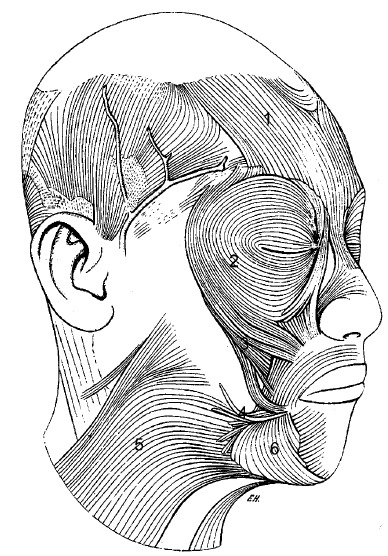
\includegraphics[width=5cm]{img/10_1.jpeg}%
			\caption{Muscles of facial expression. 1,
				frontalis; 2, orbicularis oculi; 3, zygomaticus
				major; 4, risorius; 5, platysma; 6, depressor
				anguli oris [33]}
		\end{minipage}
		\begin{minipage}[t]{.5\textwidth}
    		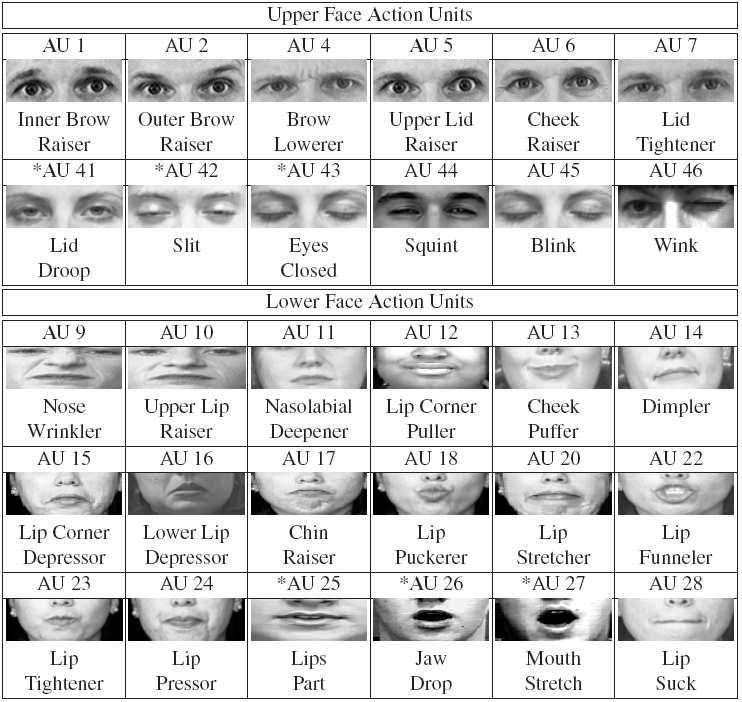
\includegraphics[width=7cm]{img/10_2.jpeg}%
			\centering
			\caption{FACS action units [35]}
		\end{minipage}
		\label{fig:example}%
	\end{figure}

	\newpage
	
% Page no 7
\subsubsection{Prototypic Emotional Expressions}
Instead of describing the detailed facial features, most FER systems attempt to recognize a small set of prototypic emotional expressions. The most widely-used set is perhaps human universal facial expressions of emotion which consists of six basic expression categories that have been shown to be recognizable across cultures \ref{fig:facialPhenotypes} .

These expressions, or facial configurations have been recognized in people from widely divergent cultural and social backgrounds, and they have been observed even in the faces of individuals born deaf and blind.

These 6 basic emotions, \textit{i.e.}, disgust, fear, joy, surprise, sadness and anger plus ``neutral'' which means no facial expression are considered in this work. Given a facial image, our system either works as a conventional classifier to determine the most likely emotion or estimates the weights (or possibility) of each emotion as a fuzzy classifier does.

	\begin{figure}[h!]
    	\centering
    	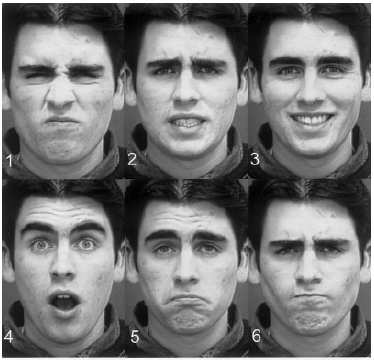
\includegraphics[width=0.5\textwidth]{img/12_1.png}
    	\caption{Basic facial expression phenotypes. 1, disgust; 2, fear; 3, joy; 4, surprise; 5, sadness; 6, anger}
    	\label{fig:facialPhenotypes}
	\end{figure}

	\section{System Structure}
	FER can be considered as a special face recognition system or a module of a face recognition system. So it should be instructive to look at the general architecture of a face recognition system. Normally, it consists of four components as depicted in \ref{fig:processingFlow}

% Page no 8
	\begin{figure}[h]
    	\centering
    	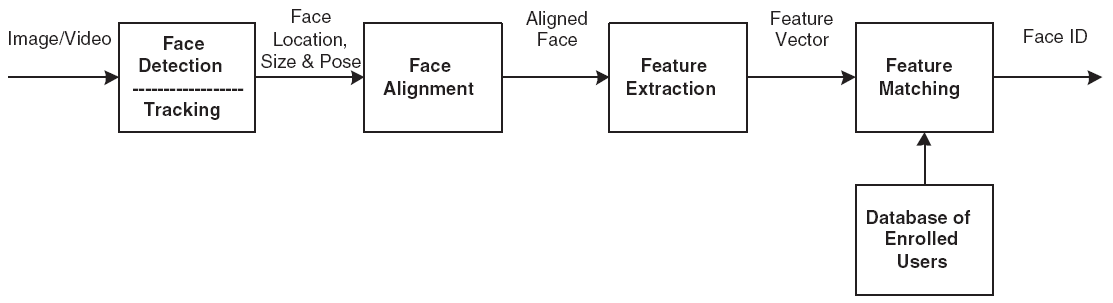
\includegraphics[width=\textwidth]{img/12_2.png}
    	\caption{Face recognition processing flow}
    	\label{fig:processingFlow}
	\end{figure}

	Face detection finds the face areas in the input image. If the input is a video, to be more efficient and also to achieve better robustness, face detection is only performed on key frames and a tracking algorithm is applied on interval frames. Face alignment is very similar to detection, but it is aimed at achieving a more accurate localization. In this step, a set of facial landmarks (facial components), such as eyes, brows and nose, or the facial contour are located; based on that, the face image is rotated, chopped, resized and even warped, this is called geometrical normalization. Usually the face is further normalized with respect to photometrical properties such as illumination and gray scale.

	Feature extraction is performed on a normalized face to provide effective information that should be useful for recognizing and classifying labels in which there is interest, such as identity, gender, or expression. The extracted feature vector is sent to a classifier and compared with the training data to produce a recognition output.

	\section{Face Detection}
	Face detection is the first step in face recognition. It has a major influence on the performance of the entire system. Several cues can be used for face detection, for example, skin color, motion (for videos), facial/head shape, and facial appearance. Most successful face detection algorithms are based on only appearance. This may be because

	\newpage
	
	% Page no - 9
	\large{appearance-based algorithms avoid difficulties in modeling 3D structures of faces. However, the variations of 3D structures due to facial expression and head pose actually heavily affect the facial appearance and make the face/non-face boundary highly complex [7]. To deal with this, a vast arrange of methods have been proposed since the 1990s.}\par
	\large{Turk and Pentland [87] describe a detection system based on eigen decomposition which is also known as principal component analysis (PCA). In their method, an image is represented by an average face plus a set of weighted “eigenfaces”. Whereas only the face images are considered in eigenface, Sung and Poggio [82] also consider the distribution of non-face images and apply Bayes’ rule to obtain a likelihood estimation. Rowley et al. [72] use neural networks and Osuna et al. [68] trained a Kernel Support Vector Machine to classify face and non-face images. In these systems, a bootstrap algorithm is iteratively used to collect meaningful examples for retraining the detector.}\par
	\large{Schneiderman and Kanade [75] use AdaBoost learning to construct a classifier based on wavelet representation of the image. This method is computationally expensive because of the wavelet transformation. To overcome this problem, Viola and Jones [93] replace wavelets with Haar features, which can be computed very efficiently [20] [80]. Their system is the first realtime frontal-view face detector [94].}\par
	\large{Under Viola’s framework, some improvements have been proposed. Lienhart et al. [52] use rotated Haar features to deal with in-plane rotation. Li et al. [51] [50] [52] propose a multiview face detection system which can also handle out-of-plane rotation using a detector-pyramid.}\par
	\large{In the following sections, we will describe two face detection algorithms: Eigenface is one of the simplest methods and Viola’s framework may be the most successful one. AdaBoost learning is an important component in Viola’s framework and this algorithm will also be useful in the feature extraction module, so our presentation focuses on this part.}
			
	\subsection{Eigenface and Template Matching}
	\large{Eigenface assumes the face image $x = (x_1,x_2,...,x_N)$ is amenable to a multivariate normal distribution from which the training images are identically independently drawn.}
	
	\newpage
	
% Page no - 10
	\large{This distribution can be described by the following probability density function:}\\
	\begin{center}
		$ f(x_1,x_2,...,x_N) = \frac{1}{(2\pi)^{N/2}|\sum_{}^{}|^{1/2}}exp(-\frac{1}{2}(x-\mu)^T\sum_{}^{-1}(x-\mu))$\\
	\end{center}
	\large{where $\sum_{}^{}$ is the covariance matrix and $\mu$ is the expectation of $x$.\\
	Eigenface decomposes $\sum_{}^{}$ using eigen decomposition as}
	\begin{center}
		$\sum_{}^{} = USU^T$\\
	\end{center}
	\large{where $U$ is a unitary matrix and $S = diag(s^2_1,s^2_2,...,s^2_N)$ is a diagonal matrix with all elements non-negative. Each column of $U, U_i,$ is called an Eigenface. A face image $x$ can be represented by $\mu$ and $U_i$ as}
	\begin{center}
		$x = \mu + \sum_{i}^{}a_iU_i$\\
	\end{center}
	\large{It can be shown that $\frac{a_i}{s_i}$ are i.i.d. standard normal variables. So the probability density function of $x$ is:}
	\begin{center}
		$f(x) = \prod_{i}^{}-\frac{1}{(2\pi)^{1/2}}exp(\frac{1}{2}\frac{a^2_i}{s^2_i}) = \frac{1}{(2\pi)^{N/2}}exp(-\frac{1}{2}\sum_{i}^{}\frac{a^2_i}{s^2_i})$\\
	\end{center}
	\large{Equation (2.4) can be used as a probability estimate and we can define a distance measure according to}
	\begin{center}
		$D = \sum_{i}^{}\frac{a^2_i}{s^2_i}$\\
	\end{center}
	\large{which is called normalized Euclidean distance. A large $D$ implies a small probability of being a face image and vice versa. Based on (2.5) Turk and Pentland [87] built a face detection system. Sung and Poggio's paper [82] used a similar idea, they assume images are produced by a mixture of Gaussian models: a face image Gaussian and a non-face image Gaussian. So they also estimate the probability of $x$ of being a non-face image $f'(x)$ and the final decision is made using a Bayesian classifier.}\\
	\large{If we further assume $\sum_{}^{}$ is an identity matrix, (2.5) degenerates into Euclidean distance which means the probability density function is controlled by, $|x - \mu|^2$, the variation of the image from the average face $\mu$. This gives the simplest detection algorithm: template matching, i.e., finding a "face template" $\mu$, and then for each $x$ determine whether it is a face image by thresholding $|x - \mu|$.}
	
% Add Page 11 - 16
	
	\newpage
	
% Page no - 17
	\begin{figure}%
		\begin{subfigure}{0.5\textwidth}
		\centering
		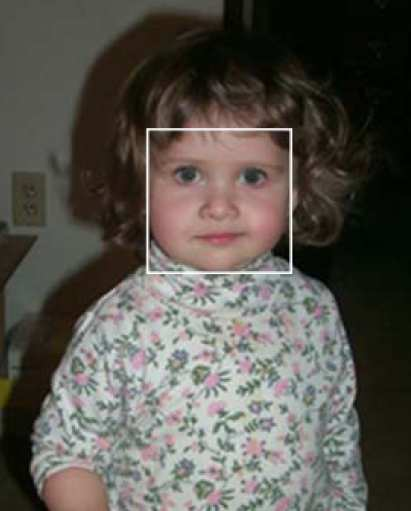
\includegraphics[width=.6\linewidth, height=0.8\linewidth]{img/17_1.png}
		\caption[label a]{Face Detection [35]}
		\label{fig:test1}
		\end{subfigure}%
		\begin{subfigure}{0.5\textwidth}
		\centering
		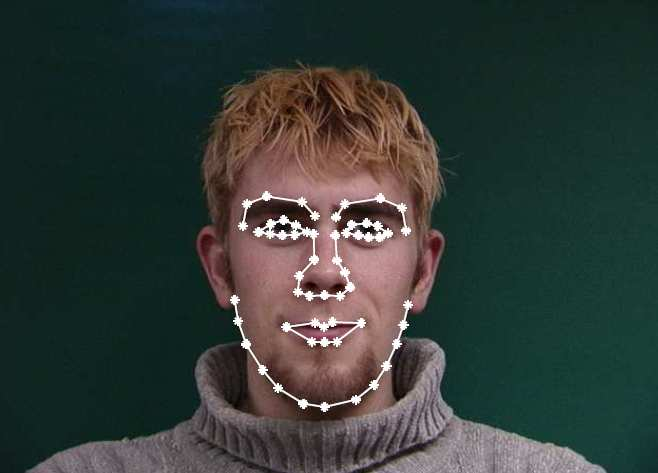
\includegraphics[width=\linewidth, height=0.8\linewidth]{img/17_2.png}
		\caption[label b]{Face Alignment [56]}
		\label{fig:test2}
		\end{subfigure}
		\caption{Detection Vs Alignment}
		\end{figure}
		
		\section{Curve Fitting}
		The basic problem of curve fitting is to locate the contour of an object in an image. Most
		curve fitting methods (explicitly or implicitly) consider two “forces”: internal force (elastic
		force) caused by deformation and external force (image force) caused by density gradient.
		As in physics, both internal force and external force cause potential energy, and the curve
		fitting is achieved by minimizing the overall energy functional (Fig.2.8).
		
		In general, a contour can be represented by c = c(s), parameterized by its arc length,
		s. The energy function can be expressed by:
		\begin{equation}
			\varepsilon = E_{elastic}(c) + E_{image}(c) = \int\limits_c (a(s)e_{elastic}(c,s) + b(s)e_{image}(c,s))ds
		\end{equation}
		
		So the optimization problem can be expressed as
		\begin{equation}
			\underset{c}{\arg\min}E_{elastic} + E_{image}(c)
		\end{equation}
		
		Usually, (2.24) is solved using iterative searching algorithms. A large number of curve
		fitting methods have been proposed using a wide range of energy functions and searching
		schemes.
	\newpage
	
% Page no - 18
	\begin{figure}[h!]
		\centering
	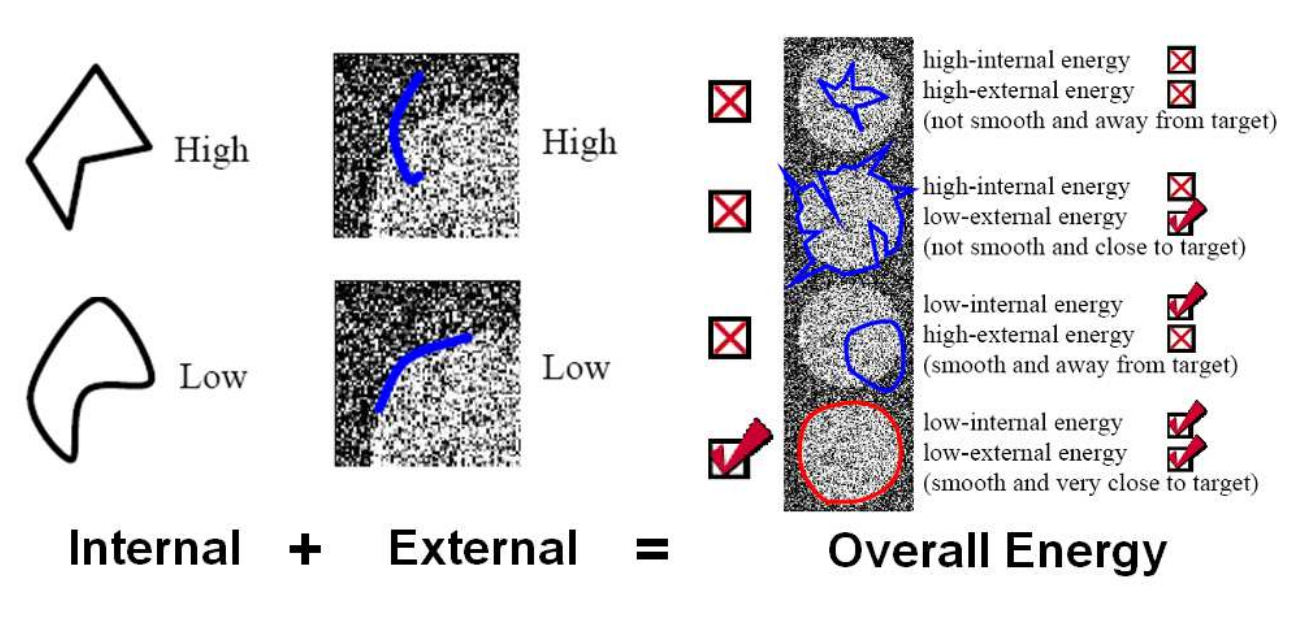
\includegraphics[width=\textwidth]{img/18_1.png}     
		\caption{Energy function and curve fitting}
		\label{fig:face}
	\end{figure}

	\paragraph{}
	It’s worth pointing out that sometimes the energy function is not explicitly given,
	instead it’s implicitly defined in the searching scheme, for example, in Active Shape Model.

	\section{Feature Extraction}
	“Feature extraction converts pixel data into a higher-level representation of shape, motion,
	color, texture, and spatial configuration of the face or its components. The extracted
	representation is used for subsequent classification. Feature extraction generally reduces
	the dimensionality of the input space. The reduction procedure should (ideally) retain
	essential information possessing high discrimination power and high stability” [14]. In the
	face recognition area, various features have been used.

	The coefficients of Eigenface can be used as features and recently, an extension of
	Eigenface [90] defines Tensorface which has shown a promising choice of feature. Active
	Appearance Model [17] decomposes the facial image into “shape” and “texture”. The shape
	vector which is coded using ASM describes the contour of the facial components, whereas
	the texture vector gives the “shape-free” facial texture. Matsuno et al. [41] extract features
	\newpage

% Page no - 19
	\noindent using a two-dimensional mesh, called Potential Net. All the above-mentioned methods are considered as holistic features, because they are related to the overall structure of the image. There is another kind of features called local features, each of which focuses only on a small region. The most straightforward idea may be to directly use image sub-windows as local features: for example, in \cite{15} Colmenarez \textit{ et al}. use nine sub-windows located around the facial components. Wavelet filters have been used too, the most popular of which is the Gabor filter which has been shown \cite{22} \cite{37} to be a reasonable model of visual processing in primary visual cortex. Yin and Wei use topographic primitive features to represent faces \cite{103}. In \cite{104}, instead of defining features ahead of time, Yu and Bhanu use a evolutionary algorithm to generate features automatically. For video-based FER, the dynamic of expression can also serve as features. \cite{44} proposes Geometric Deformation Feature which represents the geometrical displacement of certain selected landmark nodes. In \cite{1}, Aleksic and Katsaggelos use Facial Animation Parameters which are based on Active Shape Model.
	\par In this section, we'll briefly introduce some of these feature extraction methods
	\par
	\section {Tensorface}
	Tensorface \cite{90} is a multilinear extension of Eigenface. Instead of representing the face image using a linear equation.
	\begin{equation}
	x=\overline{x}+\sum_{i}a_i x_i
	\end{equation}
	It models the face by a multilinear system which is equivalent to
	\begin{equation}
	x=\overline{x}+\sum_{i_1}...\sum_{i_1}a_{i_N}...a_{i_N} x_{i_1}..._{i_N}
	\end{equation}
	\par 
	Compared to Eigenface which ignores the label of images, Tensorface analyzes a face ensemble with respect to its underlying factors(labels): for example, identities, views, and illuminations. The "principal components" in this multilinear system are referred to as Tensorfaces which are shown in Fig.2.9. The Tensorface coefficients a$_{i_k}$ can be used as features in a recognition task, and because the original image can be reproduced using 2.26, Tensorface coefficients can also be used for image synthesis where we first generate a set of coefficients, then use them to synthesize images.

% Page no - 20
	\newpage

	\par
	Since Tensorface is shown to be a promising method in face recognition, some improvements have been proposed. \cite{92} proposes Multilinear Independent Component Analysis where they try to find the independent directions of variation. In \cite{76} Shashua et al. introduce Non-Negative Tensor Factorization which is a generalization of Non-negative Matrix Factorization.
	\par 
	\begin{figure}
	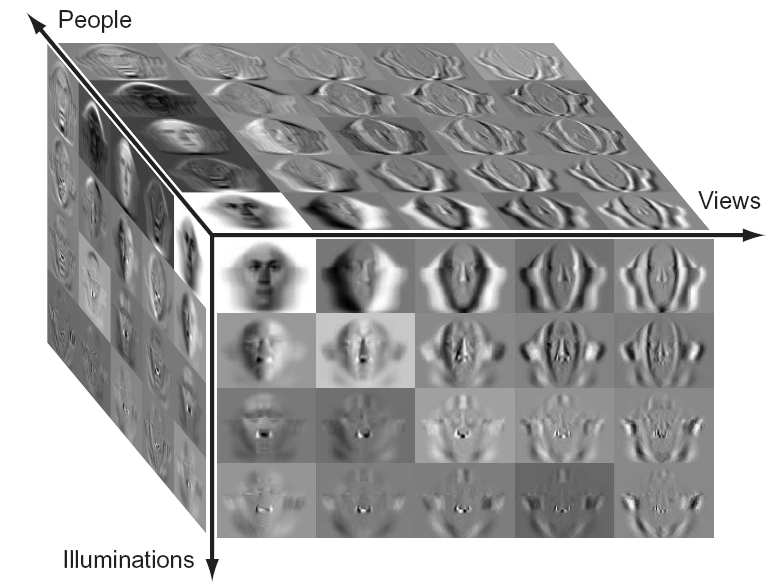
\includegraphics[width=\textwidth]{img/20_1.png}
	\caption{A partial visualization of TensorFaces bases for an ensemble of 2,700 facial images spanning 75 people, each imaged under 6 viewing and 6 illumination conditions \cite{92}}
	\label{Fig 2.9}
	\end{figure}
	\section{Potential Net}
	\par 
	Matsuno \textit{et al}. \cite{61} \cite{41} propose Potential Net to extract facial features. As shown in Fig.2.10, Potential Net is a two dimensional mesh of which nodes are connected to their four neighbors with springs, while the most exterior nodes are fixed to the frame of the Net. Similar to curve fitting, Potential Net considers two forces: each node in the mesh is driven

% Add Page 21 - 22

	\newpage

% Page no - 23
	\begin{figure}
		\centering 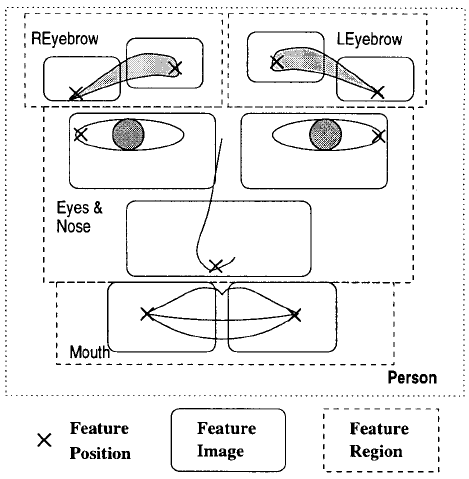
\includegraphics[totalheight=8cm]{img/93_1.png}
		\caption{Figure 2.12: Scheme of the Facial Features and Regions [15]}
		\label{Fig 2.12}
	\end{figure}
	\subsection{Support Vector Machine}
	\large{Support Vector Machine attempts to construct a linear classifier which maximizes the margin between two classes, so it’s also known as Optimal Margin Classifier [9]. Fig.2.13 gives an SVM classifier where $\frac{1}{|w|}$ gives the margin and samples along the hyper-planes are called the support vectors.}
	\par
	\large{It has been proven that SVM minimizes the Structural Risk Function which is considered as a better error estimation than the normallyused Empirical Risk Function in terms of generalization capacity.}
	\par
	\large{We consider data points of the form: $\{(x_1,y_1),...,(x_n,y_n)\}$ where $y_i$ is either 1 or -1, a label denoting the class to which the point $x_i$ belongs. The basic version of SVM can be written as}
	\newline
	\begin{center}
		$argmax\hspace{0.7cm}\frac{1}{||w||}$\\
		$\hspace{4.4cm}s.t.\hspace{0.6cm}y_i(x^Tw-b_0)\ge1,\hspace{0.3cm}\forall i$
	\end{center}
	
	\newpage
% Page no - 24
	\begin{figure}
		\centering 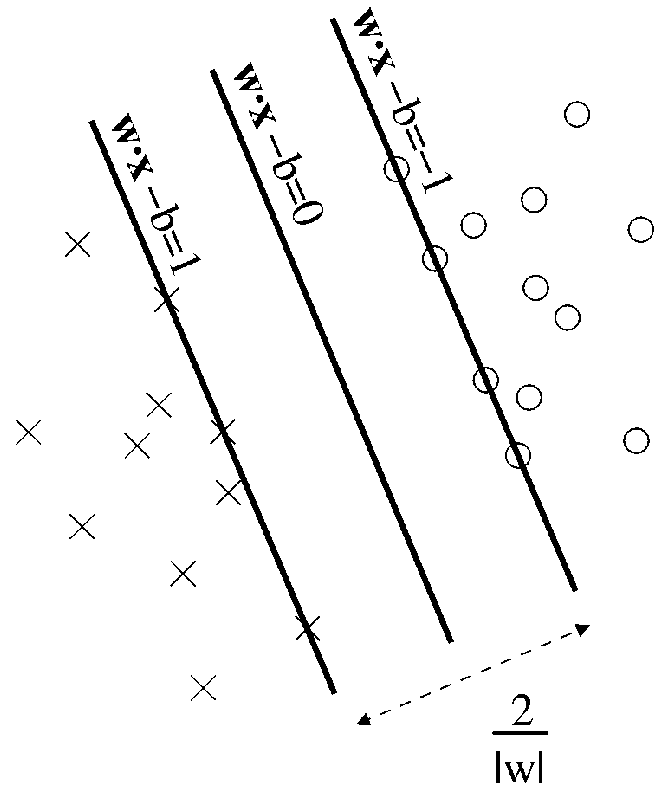
\includegraphics[totalheight=8cm]{img/93_2.png}
		\caption{Figure 2.13: Maximum-margin hyper-planes for a SVM trained with samples from two classes [99]}
		\label{Fig 2.13}
	\end{figure}
	\vspace{0.5cm}
	\large{$||...||$ in (2.27) can be replaced by any distance measure. If norm-2 is used, the problem is equivalent to}
	\begin{center}
		$argmin\hspace{0.7cm}\frac{1}{2}||w||^2$\\
		$\hspace{4.4cm}s.t.\hspace{0.6cm}y_i(x^Tw-b_0)\ge1,\hspace{0.3cm}\forall i$
	\end{center}
	\large{Equation (2.28) is a quadratic programming and according to the strong duality theorem it can be converted to:}
	\begin{center}
		$argmax\hspace{0.7cm}\sum_{i}^{}\alpha_i-\frac{1}{2}\sum_{i}^{}\sum_{j}^{}\alpha_i\alpha_jy_iy_jx^T_ix_j$\\
		$\hspace{-2.5cm}s.t.\hspace{0.6cm}\alpha_i\ge0,\hspace{0.3cm}\forall i$
	\end{center}
	\large{which is called the dual problem of (2.28).In practice, we always use (2.29) as it is easier to handle numerically. Moreover, in (2.29) all the computation of x i is written in terms of inner product, and that means it can be generalized to a nonlinear case by employing Kernel technique.}
		
	\newpage
% Page no - 25		
	\section{Face Database}
	"Because of its non rigidity and complex three-dimensional structure, the appearance of a face is affected by a large number of factors including identity, face pose, illumination, facial expression, age, occlusion, and facial hair. The development of algorithms robust to these variations requires databases of sufficient size that include carefully controlled variations of these factors. Furthermore, common databases are necessary to comparatively evaluate algorithms. Collecting a high quality database is a resource-intensive task: but the availability of public face databases is important for the advancement of the field" [35]. In this section we briefly review some publicly available databases for face recognition, face detection, and facial expression analysis, and we'll mainly focus on the three databases which we will use in this thesis. 
	\par
	To facilitate this statement, we divide face databases into two categories according to their designing goals. In the first part, we'll introduce databases which are normally used for face recognition; those which are dedicated to expression recognition will be discussed in the second part. As only a few databases are of the second type, and FER system shares some common modules with identity recognition system, in this work we also use some databases of the first type.

	\subsection{Databases For Identity Recognition}
	Most face databases are of this category (Table.2.1). To test for robustness, some of them are captured under different poses, illuminations and expressions. However, because they're mainly designed for identity recognition, the expressions are added as noise and usually not well controlled. So in general these databases are considered not suitable for FER research. In our work, we only use them to train peripheral modules (processing and Feature Extraction).

	\section*{The IMM Face Database [66]}
	The IMM Face Database comprises 240 still images of 40 individuals (7 females and 33 males), all without glasses. For each person, 6 images are provided:


	\newpage
% Page no - 26
	\begin{table}
	\caption{Some of the most popular Face Recognition Databases [35] }
	\centering
	\resizebox{14cm}{!}{
		\begin{tabular}{|c||c|c|c|c|}\hline
  			Database & No. of subjects & Pose & Illumination &Facial Expressions\\ \hline\hline
			AR & 116 & 1 & 4 & 4\\\hline
			BANCA & 208 & 1 & ++ & 1\\\hline
			CAS-PEAL & 66-1040 & 21 & 9-15 & 6\\\hline
			CMU HYPER & 54 & 1 & 4 & 1\\\hline
			CMU PIE & 54 & 1 & 4 & 1\\\hline
			Equinox IR & 91 & 1 & 3 & 3\\\hline
			FERET & 1199 & 9-20 & 2 & 2\\\hline
			Harvard RL & 10 & 1 & 77-84 & 1\\\hline
			IMM FACE & 40 & 3 & 2 & 3+\\\hline
			KFDB & 1000 & 7 & 16 & 5\\\hline
			MIT & 15 & 3 & 3 & 1\\\hline
			MPI & 200 & 3 & 3 & 1\\\hline
			ND HID & 300+ & 1 & 3 & 2\\\hline
			NIST MID & 1573 & 2 & 1 & ++\\\hline
			ORL & 10 & 1 & ++ & ++\\\hline
			UMIST & 20 & ++ & 1 & ++\\\hline
			U.Texas & 284 & ++ & 1 & ++\\\hline
			U. Oulu & 125 & 1 & 16 & 1\\\hline
			XM2VTS & 295 & ++ & 1 & ++\\\hline
			Yale & 15 & 1 & 3 & 6\\\hline
			Yale B & 10 & 9 & 64 & 1\\\hline
  
			\hline
		\end{tabular}
  	}
	\label{2.1}
	\end{table}


	\begin{itemize}
		\item Frontal face, neutral expression, diffuse light.
		\item Frontal face, happy expression, diffuse light.
		\item Face rotated approx. 30 degrees to the person’s right, neutral expression, diffuse light.
		\item Face rotated approx. 30 degrees to the person’s left, neutral expression, diffuse light.
	\end{itemize}

	\newpage
	%\onehalfspacing
	
% Page no - 27
	\begin{itemize}
		\item Frontal face, neutral expression, spot light added at the person’s left side.
		\item Frontal face, “joker image” (arbitrary expression), diffuse light.
	\end{itemize}
	\qquad The images are stored in 640 × 480 JPEG files. Owing to technique problems, most images are RGB, but some are grey-scale [66]. One good thing about this database is that manually labeled face contour is available. The following facial structures were annotated using 58 landmarks: eyebrows, eyes, nose, mouth and jaw. These landmarks are divided into seven point paths; three closed and four open as shown in Fig.2.14. In our work, this database will be used to train the ASM and AAM model.
	
	\begin{figure}[h]
		\centering
		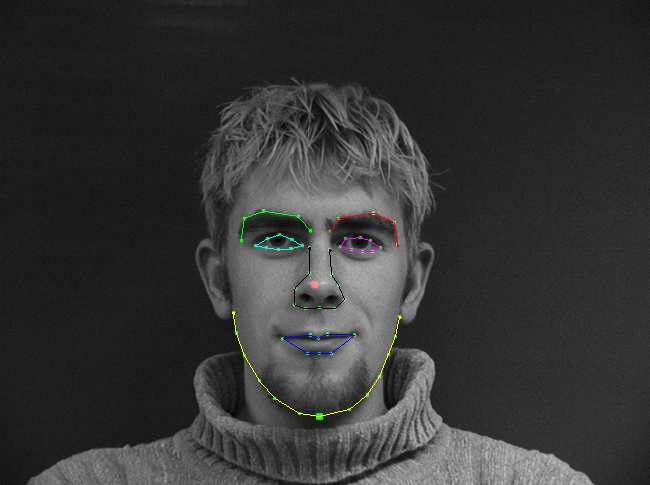
\includegraphics[scale=0.5]{img/98_1.png}
		\caption{Example image from IMM face database}
	\end{figure}
	\vspace{0.5cm}
	\noindent \textbf{CMU Pose, Illumination, and Expression Database [79]} \vspace{0.3cm} \\
	The CMU-PIE database is among the most comprehensive databases in this area. It systematically samples a large number of pose and illumination conditions along with a variety of facial expressions. The PIE database was captured under 21 illuminations (lit by 21 flashes) from 13 directions (using 13 synchronized cameras). In total, there are 41,368 images obtained from 68 individuals. In our experiment, we only use a sub-set of this database which consists of images of 62 people. 25 images were selected for each individual
	
	\pagebreak
	
% Page no - 28	
	\noindent with 5 different viewpoints and 5 different illuminations. Part of the data set is shown in Fig.2.15.
	
	\begin{figure}[h]
		\centering
		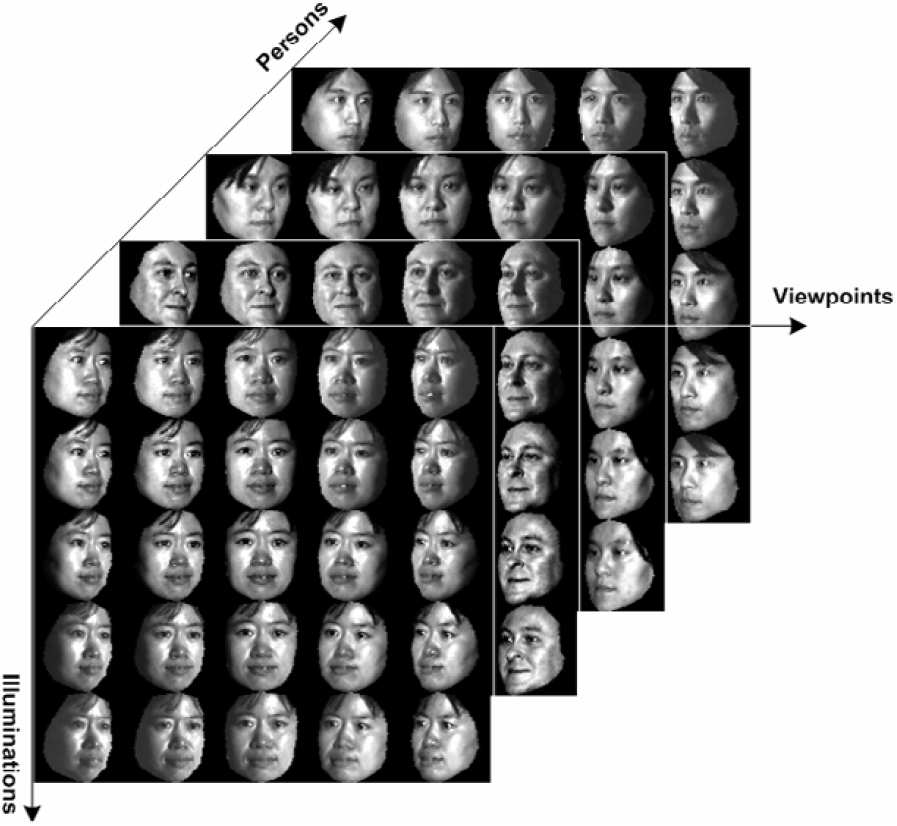
\includegraphics[scale=0.3]{img/98_2.png}
		\caption{A subset of CMU PIE database [53]}
	\end{figure}
	\vspace{0.5cm}
	
	\noindent \textbf{\large \subsection{Databases for Expression Recognition}} \vspace{0.3cm}
	"The human face is able to display an astonishing variety of expressions. Collecting a database that samples this space in a meaningful way is a difficult task" [35]. As a result, there are many fewer databases available for expression recognition (Table 6.1). As mentioned in 2.1.1, there are two ways to describe facial expressions. Available databases can be categorized into two classes according to the description they used. In one group [38] expressions are coded in FACS, while in the other group [57] images are labeled by their sprototypic emotional expressions.
	\vspace{0.1cm} \\
	
	\noindent \textbf{Japanese Female Facial Expression Database [57]}
	\vspace{0.3cm} \\
	The JAFFE database contains 213 images of 10 Japanese female models. Their images are labeled by emotions: six basic emotions (anger, disgust, fear, joy, happy, sad and surprise) are considered and “Neutral” is added as the 7th emotion which is defined through the absence of expression. Fig.2.16 shows example images for one subject along with emotion

	\newpage
	
% Page no - 29
	\begin{table}
		\caption{Commonly used expression recognition databases [35] }
  		\centering
  		\resizebox{14cm}{!}{
  			\begin{tabular}{c||l|c|c|c}
  				Database & No. of subjects & No. of Expressions & 						Image Resolution & Video/Image\\ \hline\hline
  				JAFFE & 10 & 7 & 256 X 256 & Image\\\hline
  				U. Maryland & 40 & 6 & 560 X 240 & Video\\\hline
  				Cohn-Kanade & 100 & 23 & 640 X 480 & Video\\\hline
  			\end{tabular}
  		}
	\end{table}

	labels. The images were originally printed in monochrome and then digitized using a flatbed scanner.
	
	\begin{figure}
		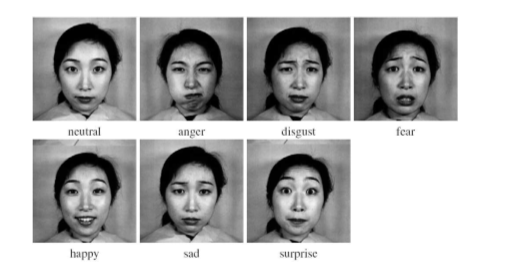
\includegraphics[width=\textwidth]{img/94_1.jpg}
		\caption{Example images from JAFFE database[35]}
		\label{Fig 2.16}
	\end{figure}
	\section{Chapter Summary}
	\par
	In this chapter, we first talked about the background of facial analysis, then gave an overview of the development in this area, and we also briefly introduced some state of the art techniques which might be useful for our system. At the end, we had a glance at some face databases for identity and expression recognition. Starting in the next chapter, we'll discuss the design of our FER system.
	\end{document}

\end{document}